Der Aufbau setzt sich aus den folgenden Bestandteilen zusammen: ein Funktionsgenerator mit regelbarer Frequenz $f$, eine Brückenschaltung mit regelbarem Widerstand $R$, den Messspulen und einer Öffnung für die Proben, ein Selektivfilter mit regelbarem Verstärker, ein Linearverstärker, ein Oszilloskop mit Millivoltmeter und die Proben.
Zunächst wird die Ausgangsspannung des Funktionsgenerators geprüft, da der Selektivverstärker nicht mehr als $U=\SI{1}{V}$ gespeist bekommen darf.
Dafür wird der Funktionsgenerator mit dem Oszilloskop verbunden.
Die Filterkurve des Selektivfilters wird ausgemessen.
Dazu wird der Funktionsgenerator mit dem Selektivfilters verbunden.
Der Selektivfilter wird an das Oszilloskop mit Millivoltmeter geschlossen.
Gemessen wird die maximale Ausgangsspannung $U_A$ am Oszilloskop in Abhängigkeit der vom Funktionsgenerator erzeugten Frequenz $f$.
\\Für die Messung der Suszeptibilität wird die Schaltung geändert (Abb. \ref{fig:aufbau}).
\begin{figure}[h!]
  \centering
  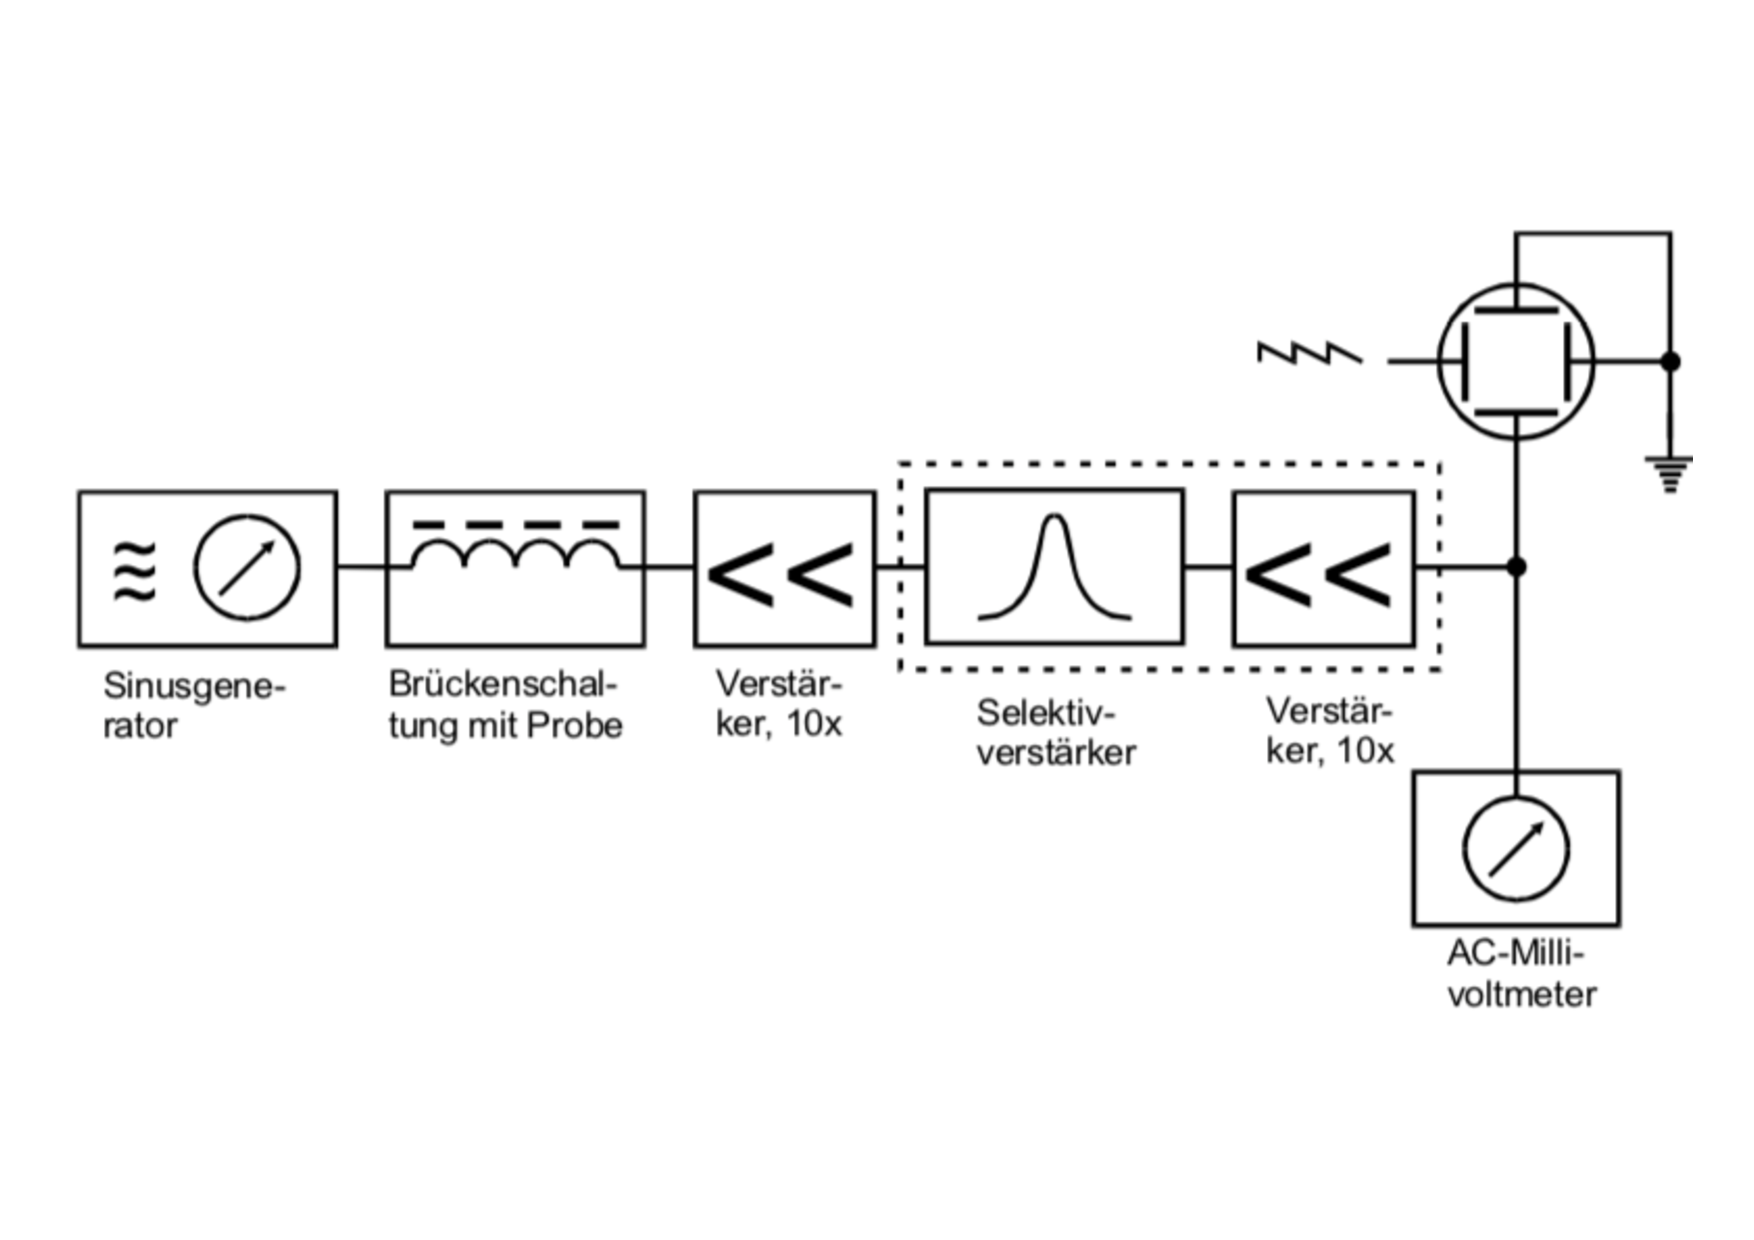
\includegraphics[width=\textwidth]{606aufbau.pdf}
  \caption{Aufbau der Messapparatur \cite{1}}
  \label{fig:aufbau}
\end{figure}
Der Funktionsgenerator wird mit der Brückenschaltung verbunden.
Die Brückenschaltung wird mit dem Linearverstärker vernetzt.
Der Linearverstärker wird an den Selektivfilter geschaltet.
Am Selektivfilter wird die Verstärkung $\times 10$ gewählt.
Der Selektivfilter wird anschließend mit dem Millivoltmeter verbunden.
Als Frequenz der Spannung wird der Hochpunkt der Filterkurve gewählt.
Nun wird der regelbare Widerstand so lange verändert, bis die Ausgangsspannung auf dem Millivoltmeter ein Minimum erreicht.
Die AUsgangsspannung und der Widerstand werden notiert.
Nun wird die Probe in die Spule eingeführt.
Erneut wird mit dem regelbaren Widerstand das Minimum der Ausgangsspannung gesucht.
Die Ausgangsspannung und der Widerstand werden notiert.
Die Messung wird drei mal wiederholt.
